\chapter{Energy-Based Models (EBM)}

Gli \textbf{Energy-Based Models} (EBM) costituiscono un paradigma di modellazione che si distacca dai classici approcci discriminativi o generativi che conosciamo. Invece di apprendere direttamente una funzione esplicita di predizione normalizzata, un \textbf{EBM} definisce un'\textit{energia} associata a ogni configurazione possibile di input $x$ e output $y$, misurandone la compatibilità. Questa energia viene definita tramite una funzione scalare $E(x, y)$, il quale obbiettivo è minimizzarla, definito come \textit{obbiettivo inferenziale}. Gli \textbf{Energy Based Model}, si articolano principalmente in due fasi, quella di allenamento, solitamente molto costosa e quella di inferenza. 

\section{Training}
Nella prima fase, il modello impara la funzione d'energia tramite l'uso di un input e di un'etichetta di riferimento, l’idea chiave è definire un’energia associata a ogni configurazione possibile degli input, dove le configurazioni "plausibili" hanno energia bassa mentre le configurazioni "implausibili" hanno energia alta. Allenare un EBM richiede minimizzare un loss che coinvolge questa energia, spesso confrontando l’energia di esempi reali con quella di esempi generati.
\section{Inferenza}
Una volta che il modello è stato allenato, possiamo usarlo per fare inferenza, ossia determinare quale output y (o quale input x) minimizza l’energia, in altre parole, trovare la configurazione più probabile secondo il modello. Ad esempio, in un EBM discriminativo $E(x,y)$, possiamo usare il modello per inferire l’etichetta $y$ più probabile per un dato $x$:

\begin{equation}
    \hat{y} = \arg\min_y E(x, y)
\end{equation}
In molti casi pratici il modello EBM è già allenato da qualcun altro, e noi lo usiamo solo per inferneza, cioè non modifichiamo i pesi, ma utiliziamo il modello per selezionare le configurazioni a bassa energia, ad esempio:
\begin{itemize}
    \item Trovare la label più probabile per un'immagine;
    \item Campionare un'immagine simile a un target;
    \item Scegliere tra alternative quella più compatibile con un certo contesto.
\end{itemize}

Il fenomeno dell'inferenza viene solitamente visualizzato tramite un'interpretazione grafica visibile in Figura~\ref{fig:InfGoodBad}. Se la superficie è piatta, l'allenamento non è stato fatto in maniera corretta, poiché non identificherà delle differenze nelle varie zone. Se invece la superficie risulta essere ricurva, è stato allenato bene, distinguendo varie zone in base alla loro energia. Il passo successivo sarà semplicemente quello di trovare i valori precisi che generano il minimo.
\begin{figure}
    \centering
    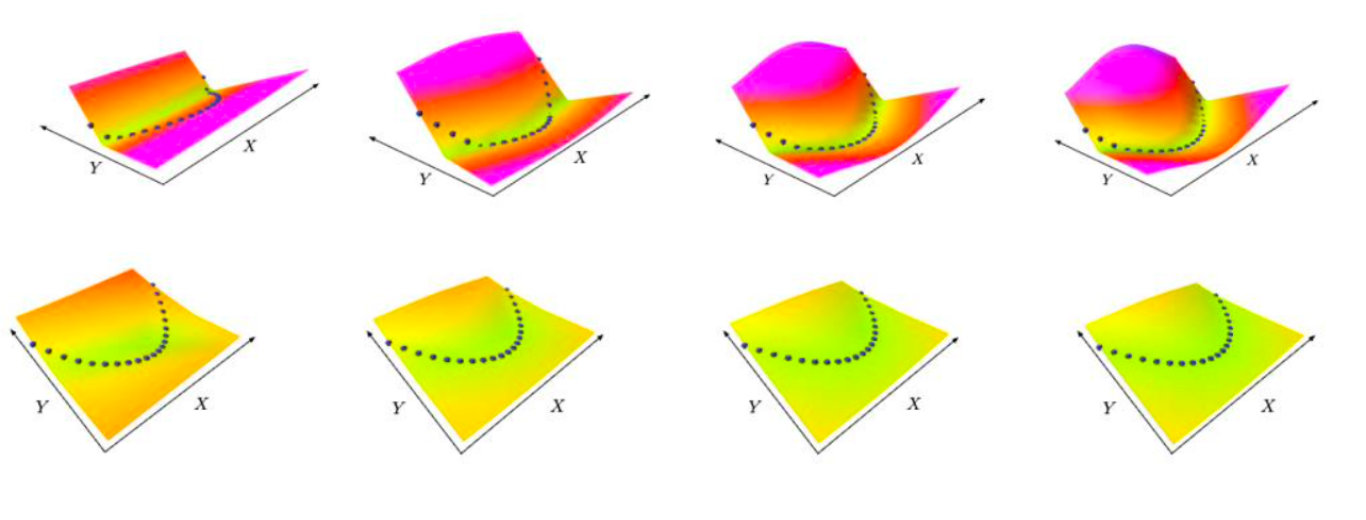
\includegraphics[width=0.7\textwidth]{figure/InferenceGoodBad.png}
    \caption{Applicazione dell'inferenza a seguito di un buon training (sopra), e l'esito a seguito di un pessimo training (sotto).}
    \label{fig:InfGoodBad}
\end{figure}

\subsection{Quando usare un EBM}
I casi d'uso degli EBM includono:
\begin{itemize}
    \item Problemi che richiedono calcoli complessi per determinare l'output;
    \item Situazioni con uscite multiple plausibili;
    \item Inferenza come soddisfacimento di vincoli, tipico di traduzioni linguisticamente corrette o trascrizioni fonetiche coerenti.
\end{itemize}

\section{Modelli espliciti vs impliciti}

Un modello feed-forward classico è una funzione esplicita $y = f(x)$, dunque calcola $y$ a partire da $x$, mentre un EBM definisce una relazione \textit{implicita} tra $x$ e $y$ tramite la funzione energetica $E(x, y)$. L'inferenza consiste nel risolvere l'ottimizzazione rispetto a $y$. Questo consente l'esistenza di molteplici $y$ compatibili con uno stesso $x$, rendendo l'approccio adatto per compiti multimodali, se $y$ è continuo, è essenziale che $E$ sia differenziabile e liscia, per consentire l'uso di algoritmi di ottimizzazione basati sul gradiente.

\begin{figure}
    \centering
    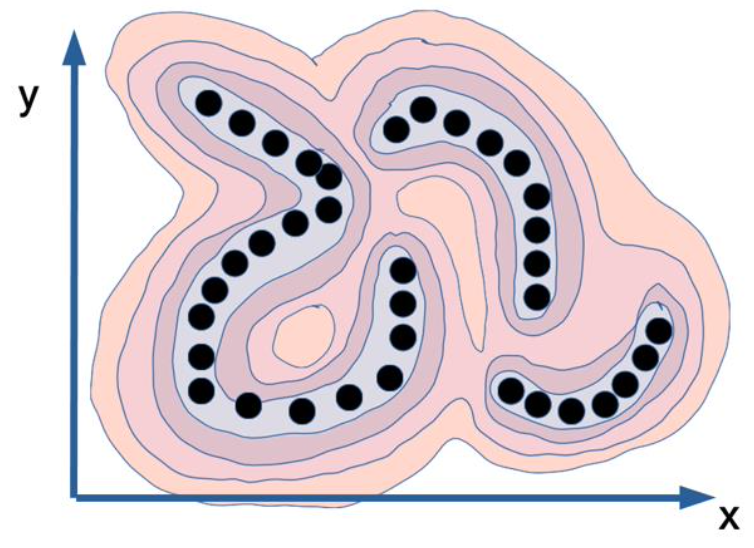
\includegraphics[width=0.7\textwidth]{figure/LowEnHighEn.png}
    \caption{Visualizzazione dell'energia, vicino ai datapoint abbiamo un'energia più bassa, mentre man mano che ci si allontana l'energia aumenta.}
    \label{fig:lEnhEn}
\end{figure}

\section{EBM per predizione multimodale}

Due degli approcci più utilizzati, ma diversi fra loro che estendono il paradigma classico degli EBMs, sfruttati in ambiti come multimodalità e modellazione generativa profonda, sono i seguenti:

\begin{itemize}
    \item \textbf{Joint Embedding Architectures:} basate sulla distanza nello spazio delle feature;
    \item \textbf{Latent Variable Models:} introducono variabili latenti per rappresentare fattori di variazione non osservati.
\end{itemize}

\subsection{Joint Embedding}

In un \textbf{Joint Embedding} EBM, si definisce una funzione di energia sullo spazio latente condiviso tra input e output, tipicamente tramite embedding. È utilizzato in modelli contrastivi e multimodali, algoritmi noti includono Siamese Networks e tecniche di metric learning~\cite{bromley1993signature, chopra2005learning, hadsell2006dimensionality}. Il vantaggio principale è l'assenza di necessità di ricostruzione a livello di pixel. Considerando $x$ come un'immagine di input e $y$ come output testuale e $f(x)$ e $g(y)$ due reti neurali, esse proiettano $x$ e $y$ in uno spazio comune nella seguente maniera:

\begin{equation}
    E(x,y) = - \langle f(x)\,,\,g(y)\rangle
\end{equation}

L'energia pertanto viene ottenuta come il prodotto scalare o cosine similarity delle due reti, l'energia risulterà di basso valore se $x$ e $y$ risultassero compatibili fra loro, fornendo una forte similarità. Esempi reali di applicazione includono:
\begin{itemize}
    \item DeepFace~\cite{taigman2014deepface};
    \item PIRL~\cite{misra2019pirl}, MoCo~\cite{he2019moco};
    \item SimCLR~\cite{chen2020simclr}.
\end{itemize}

L'obbiettivo finale è ovviamente quello di minimizzare l'energia e dunque massimizzare la similarità per le coppie vere, mentre massimizzare l'energia e minimizzare la similarità per le coppie false.

\subsection{Latent Variable EBMs}
In questa tipoliga di modello vengono sfruttate le variabili latenti $z$, le quali parametrizzano lo spazio delle predizioni. Idealmente rappresentano dei fattori indipendenti, tuttavia la loro capacità informativa deve essere minimizzata in modo tale da evitare che tutta l'informazione della predizione passi da $z$, ma venga solo influenzata parzialmente da essa.

\begin{figure}
    \centering
    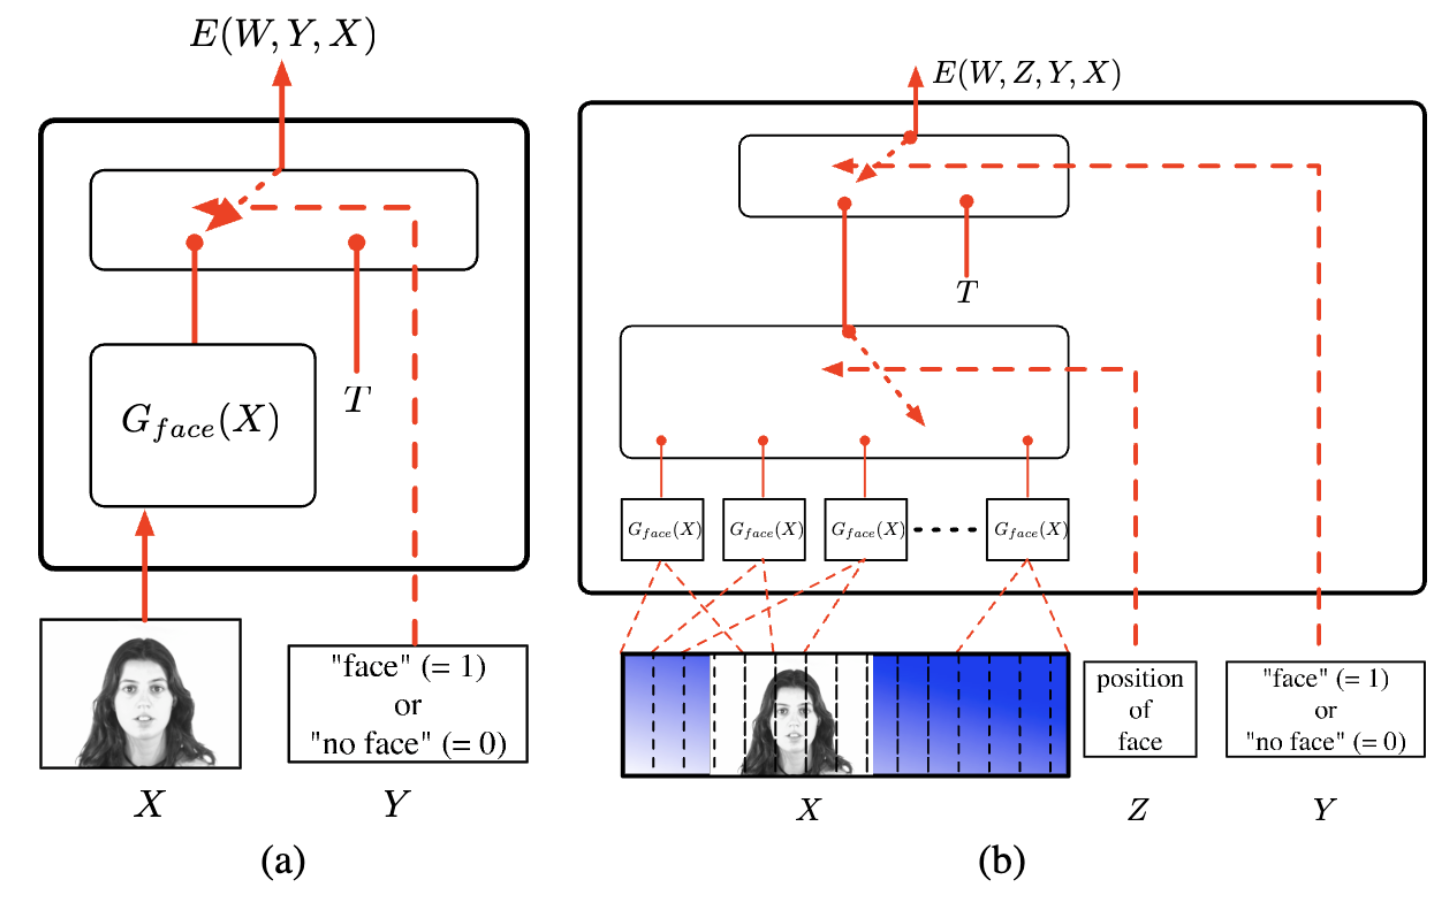
\includegraphics[width=0.6\textwidth]{figure/ebm-face.png}
    \caption{Confronto tra due architetture Energy-Based: (a) un EBM discriminativo semplice, e (b) un EBM con variabile latente. 
    Nel primo caso, la funzione di energia $E(W, Y, X)$ valuta direttamente la compatibilità tra l'immagine $X$ e l'etichetta binaria $Y$. Nel secondo caso, viene introdotta una variabile latente $Z$ che rappresenta la posizione del volto, e il modello calcola l'energia congiunta $E(W, Z, Y, X)$. Questo consente al modello di apprendere rappresentazioni strutturate e di migliorare la localizzazione e classificazione del volto all'interno dell'immagine.}
    \label{fig:ebm-face}
\end{figure}

Alcuni esempi applicativi di questa tipologia di modello si riversano nella lettura di parole scritte a mano, permettendo di sapere dove iniziano e finiscono i caratteri di una parola, ma anche nella comprensione del parlato, riuscendo a segmentare in fonemi o parole all'interno di un discorso.

\subsection{EBM con variabili latenti condizionali}
Come abbiamo detto precedentemnte nel modello con variabili latenti, vi è il rischio che la variabile latente prenda il soppravvento sulle informazioni fornite in input, pertanto è utile introdurre un regolarizzatore $R(z)$ che limiti la capacità informativa di $z$. Altrimenti, ogni $y$ potrebbe essere ricostruito perfettamente, risultando in una superficie energetica piatta. Alcuni approcci includono:
\begin{itemize}
    \item Quantizzazione/discretizzazione;
    \item Penalizzazioni tipo L0, L1;
    \item Inibizione laterale;
    \item Aggiunta di rumore controllato.
\end{itemize}

\section{Training degli Energy-Based Models}

L’addestramento di un \textbf{Energy-Based Model} (EBM) consiste nel parametrizzare una funzione di energia $F(x, y; \theta)$ in modo che a ogni coppia di input $(x, y)$ venga associato un valore di energia. L’obiettivo è che le coppie corrette (quelle osservate nei dati) abbiano energia più bassa rispetto a tutte le altre combinazioni possibili:
\begin{equation}
    F(x^{(i)}, y^{(i)}) < F(x^{(i)}, y), \quad \forall y \neq y^{(i)}
\end{equation}
In questo modo, il modello impara una funzione energetica che distingue correttamente le coppie plausibili da quelle implausibili.
\subsection{Due approcci principali}
L’addestramento di un EBM può essere condotto secondo due famiglie principali di metodi:
\begin{enumerate}
    \item \textbf{Metodi contrastivi:} minimizzano l’energia associata alle coppie corrette e la massimizzano per le coppie errate. Esempi includono la \textit{Contrastive Divergence} e le \textit{margin-based loss};
    \item \textbf{Metodi con regolarizzazione o architetturali:} invece di modellare esplicitamente coppie negative, questi metodi impongono vincoli sulla forma di $F$ o penalizzano regioni troppo ampie a bassa energia, garantendo una funzione più liscia e generalizzabile.
\end{enumerate}

\subsection{Problemi con il massimo di verosimiglianza}
L’approccio probabilistico tradizionale agli EBM mira a modellare la distribuzione dei dati tramite la massimizzazione della verosimiglianza. Tuttavia, questo equivale a creare un “canyon” infinitamente stretto e profondo attorno alla distribuzione dei dati osservati. Un tale scenario porta a due problematiche principali:
\begin{itemize}
    \item La funzione energetica diventa troppo \textbf{non liscia}, rendendo difficile la discesa del gradiente;
    \item Il modello tende a \textbf{overfittare}, concentrandosi eccessivamente sui dati osservati.
\end{itemize}

Per questo motivo, spesso si preferiscono approcci \textbf{regolarizzati o contrastivi}, che mantengono una funzione energetica più stabile.

\subsection{Distribuzione di Gibbs}
In un’ottica probabilistica, la funzione di energia può essere interpretata come il negativo del logaritmo di una distribuzione non normalizzata:
\begin{equation*}
    P(y|x) \propto e^{-\beta F(x, y)}.
\end{equation*}
dove:
\begin{itemize}
    \item $\beta$ è un parametro di scala chiamato \textit{Inverse Temperature};
    \item $F(x,y)$ è l'energia associata alla coppia $(x,y)$;
\end{itemize}

Il termine di normalizzazione (partizione di Gibbs) è dato da:

\begin{equation}
    Z(x)=\int_{y'}e^{-\beta\,F(x,y')}dy'
\end{equation}

che però risulta essere molto costoso da calcolare, poiché richiede di sommare (o integrare) su tutte le possibili $y'$.
Per questo, nella pratica si evita di stimare $P(y|x)$ in forma esplicita, e si preferiscono strategie di ottimizzazione basate su confronti di energia.
\section{Contrastive Methods}

I \textbf{metodi contrastivi} addestrano il modello riducendo l’energia per le coppie corrette e aumentandola per tutte le altre.
In termini probabilistici, si può scrivere:

\begin{equation}
    P(Y\,|\,W)= -\frac{e^{-\beta\,E(Y,W)}}{\int_{y'}e^{-\beta\,E(y,W)}}
\end{equation}
e la funzione di perdita corrispondente è:
\begin{equation}
    L(Y,W) = E(Y,W) + \frac{1}{\beta}\,\log\int_ye^{-\beta\,E(y,W)}dy'
\end{equation}

La prima parte riduce l’energia dei campioni corretti, mentre la seconda penalizza il modello se assegna energia bassa anche ad altre configurazioni.

\subsection{Esempi di contrastive training}
\begin{itemize}
    \item \textbf{Contrastive Divergence (CD):} si utilizza un set di campioni reali e un set di campioni “negativi” generati tramite catene di Markov (MCMC).
    \item \textbf{Loss a margine:} funzioni come la \textit{Square-Square loss} o la \textit{negative log-likelihood} introducono un margine esplicito tra energia positiva e negativa.
    \item \textbf{Embedding contrastivo:} nello spazio delle feature, i campioni positivi vengono spinti vicini e quelli negativi allontanati.
\end{itemize}

\section{Embedding non contrastivo}

Gli \textbf{embedding non contrastivi} superano la necessità di generare "esempi negativi" o di effettuare \textit{negative mining}.
Essi utilizzano due reti quasi identiche (una principale e una "target") con pesi lievemente diversi, aggiornati con strategie lente o mediate.Esempi noti:
\begin{itemize}
    \item \textbf{SimSiam}~\cite{chen2021simsiam};
    \item \textbf{BYOL} (\textit{Bootstrap Your Own Latent}).
\end{itemize}

Questi metodi si basano sull’idea che un modello possa auto-supervisionarsi, imparando rappresentazioni coerenti da due viste diverse dello stesso campione, anche senza etichette o esempi negativi espliciti. Non trattiamo questi esempi, poiché porterebbero a un livello di dettaglio ulteriore, il quale porterebbe ad andare al di fuori delle competenze richieste dal corso, tuttavia possono essere approfonditi attraverso la lettura dei paper citati.

\section{Self-Supervised Learning (SSL)}
Il \textbf{Self-Supervised Learning} nasce dall’osservazione del modo in cui gli esseri umani, da bambini, apprendono: esplorando l’ambiente e costruendo internamente rappresentazioni del mondo a partire da osservazioni parziali. Un modello SSL impara a:
\begin{itemize}
    \item Predire parti mancanti o corrotte dell’input a partire dalle parti osservate;
    \item Ricostruire dati incompleti o rumorosi;
    \item Comprendere relazioni temporali o spaziali implicite.
\end{itemize}

In altre parole, l’obiettivo è imparare una rappresentazione utile del mondo senza etichette, sfruttando solo la struttura dei dati.

\subsection{Applicazioni di SSL}
Esempi moderni di apprendimento self-supervised includono:
\begin{itemize}
    \item \textbf{Wav2Vec 2.0:} addestrato su 960 ore di parlato non etichettato, ottiene prestazioni simili a modelli supervisionati che richiedono 100 volte più dati etichettati;
    \item \textbf{BERT} e \textbf{GPT}: basati sulla predizione di token mascherati o successivi, hanno rivoluzionato il NLP mostrando come la predizione contestuale possa generare rappresentazioni linguistiche estremamente potenti.
\end{itemize}

Le performance su benchmark come RACE dimostrano che i modelli SSL possono raggiungere accuratezze tra il 45\% e il 90\%, pur essendo addestrati senza supervisione esplicita.
